\documentclass[letterpaper,11pt]{article}

% Soporte para los acentos.
\usepackage[utf8]{inputenc}
\usepackage[T1]{fontenc}    
% Idioma español.
\usepackage[spanish,mexico, es-tabla]{babel}
% Soporte de símbolos adicionales (matemáticas)
\usepackage{multirow}
\usepackage{amsmath}		
\usepackage{amssymb}		
\usepackage{amsthm}
\usepackage{amsfonts}
\usepackage{latexsym}
\usepackage{enumerate}
\usepackage{ragged2e}
\usepackage{graphicx}
% Modificamos los márgenes del documento.
\usepackage[lmargin=2cm,rmargin=2cm,top=2cm,bottom=2cm]{geometry}

\title{Facultad de Ciencias, UNAM \\ Redes Neuronales \\ 
       \textit{The Art of Nomography I: Geometric Design}}
\author{Rubí Rojas Tania Michelle}
\date{24 de marzo de 2020}

\begin{document}
\maketitle
Este ensayo habla sobre la descripción general de cómo funcionan los
\textit{nomogramas} y cómo se construyen desde cero. Esta primer parte, en 
particular, aborda los diseños a escala recta. 

La \textit{Nomografía} es la representación gráfica de las relaciones o leyes
matemáticas. Fue inventada en $1880$ por \textit{Phillbert Maurice d'Ocagne} y
fue utilizada ampliamente por ingenieros ya que gracias a éstas se podían 
realizar cálculos gráficos (rápidos) de fórmulas complicadas con una precisión 
práctica. 

Junto con las matemáticas involucradas, se utilizó mucho ingenio en el diseño
de los nomogramas para aumentar su utilidad y precisión. Se escribieron varios
libros sobre \textit{nomografía}, pero con la difusión de las calculadoras y 
computadoras, eventualmente comenzaron a desaparecer (muy rara vez aparece un 
\textit{nomograma} en un \textit{entorno moderno}). La teoría de los 
\textit{nomogramas} "se basa en todos los aspectos de la geometría analítica,
descritiva y proyectiva, los diversos campos del álgebra y otros campos 
matemáticos" $[$Douglas$]$.

La forma más simple de \textit{nomograma} es una escala tipo Fahrenheit vs. 
Celsius vista desde un termómetro analógico o una tabla de conversión. El 
espacio lineal se puede reemplazar con el espacio logarítmico para manejar las
conversiones que involucran potencias. Una regla de cálculo (considerada también
como un \textit{nomograma}) está diseñada para proporcionar operaciones 
aritméticas básicas con el fin de resolver una amplia variedad de ecuaciones 
con una secuencia de pasos, mientras que el \textit{nomograma tradicional} está 
diseñado para resolver una ecuación específica en un sólo paso. 

La mayoría de los \textit{nomogramas} aquí presentados son las formas clásicas
que consisten en tres o más escalas rectas o curvas, cada una representando una 
función de una sola variable que aparece en una ecuación. Una regla, llamda 
\textit{línea de índice}, se coloca a través de estas escalas a valores 
conocidos de estas variables, y el valor de una variable desconocida se 
encuentra en el punto cruzado en esa escala. Esto proporciona un medio analógico
para calcular la solución de una ecuación que involucra una incógnita.

\begin{enumerate}
    \item \textbf{La geometría de los nomogramas}
    
    Podemos diseñar \textit{nomogramas} compuestos de escalas rectas mediante 
    el análisis de sus propiedades geométricas, y se puede constuir una variedad 
    de nomogramas interesantes a partir de éstas derivaciones (éstos son los 
    más frecuentes). 

    El siguiente gráfico 
    \begin{figure}[htb]
        \centering
        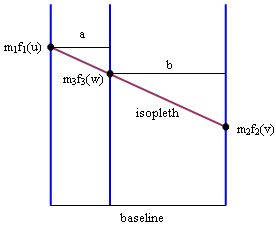
\includegraphics[width=0.2\textwidth]{./imagenes/geometry1.jpg}
    \end{figure} 

    muestra un \textit{nomograma} básico de escala paralela para calcular 
    \begin{equation*}
        f_{1} (u) + f_{2} (v) = f_{3} (w)
    \end{equation*}

    Cada función representada es una escala vertical que utiliza un factor de 
    escala correspondiente (también llamado \textit{módulo de escala}) a 
    $m_{1}, m_{2}$ o $m_{3}$, el cual proporciona un \textit{nomograma} de 
    tamaño conveniente. El espaciado de las líneas se muestra como $a$ y $b$. 
    Por triángulos similares, tenemos que 
    \begin{equation*}
        \frac{[m_{1} f_{1} (u) - m_{3} f_{3} (w)]}{a} = 
        \frac{[m_{3} f_{3} (w) - m_{2} f_{2} (v)]}{b}
    \end{equation*}

    el cual puede ser reorganizado como 
    \begin{equation*}
        m_{1} f_{1} (u) + (\frac{a}{b}) m_{2} f_{2} =
        (1 + \frac{a}{b}) m_{3} f_{3} (w)
    \end{equation*}

    Entonces, para llegar a la ecuación original tenemos que cancelar todos los 
    términos que involucran a $m, a$ y $b$, lo cual se logra al establecer
    \begin{equation*}
        m_{1} = (\frac{a}{b}) m_{2} = (1 + \frac{a}{b}) m_{3}
    \end{equation*}

    La mitad izquierda de esta relación proporciona la escala relativa de las 
    dos escalas externas y las partes externas proporcionan la escala de la 
    escala media 
    \begin{equation*}
        \frac{m_{1}}{m_{2}} = \frac{a}{b m_{3}} = \frac{m_1 m_2}{m_1 + m_2}
    \end{equation*} 

    Hay que tener en cuenta que la línea de base no tiene que ser perpendicular
    a las escalas para que la proporción de triángulo similar sea válida. 

    Ahora $a = b$ para el caso donde la escala media se encuentra a medio camino
    entre las escalas externas (en este caso $m_1 = m_2$ y $m_3 = 
    \frac{m_2}{2}$). Para un rango más pequeño y una mayor precisión para una 
    escala externa, podemos cambiar su escala $m$ y mover la línea media lejos 
    de ella y hacia la otra escala externa. De hecho, si la escala desconocida 
    $W$ tiene un rango muy pequeño, se puede mover afuera de las otras dos 
    escalas para ampliar la escala. Las adiciones a $u, v$ o $w$ simplemente
    desplazan los valores de la escala hacia arriba o hacia abajo. Los 
    multiplicadores de $u, v$ y $w$ multiplican el valor al dibujar escalas (no 
    se incliyen en los valores de $m$ de los cálculos anteriores). Restar un 
    valor simplemente invierte la dirección arriba/abajo de la escala, y si dos 
    valores son negativos, sus escalas simplemente pueden intercambiarse. Un 
    ejemplo de ésto se representa en el siguiente \textit{nomograma}:
    \begin{figure}[htb]
        \centering
        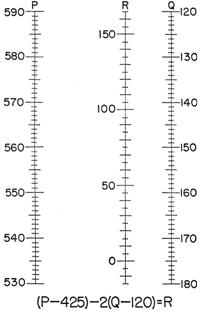
\includegraphics[width=0.2\textwidth]{./imagenes/image004.jpg}
        \caption{Nomograma de escala paralela para $(u - 425) - 2(v - 120) = w$}
    \end{figure} 

    Trazar escalas logarítmicas en lugar de lineales expande el uso de 
    \textit{nomogramas} de escala paralela a ecuaciones muy complicadas. El uso
    de logaritmos permite que las multiplicaciones se representen mediante 
    adiciones y las potencias se representen mediante multiplicaciones de
    acuerdo con las siguientes reglas:
    \begin{equation*}
        \log (cd) = \log (c) + \log (d)
    \end{equation*}

    \begin{equation*}
        \log c^d = d \log c
    \end{equation*}

    Por lo que, si tenemos una ecuación de la forma 
    \begin{equation*}
        f_1 (u) \times f_2 (v) = f_3 (w)
    \end{equation*}

    entonces podemos reemplazarla con 
    \begin{equation*}
        \log [f_1 (u) \times f_2 (v)] = \log f_3 (w)
    \end{equation*}

    Así convertimos la ecuación original en una sin multiplicación de variables.
    Tengamos en cuenta que no hay necesidad de resolver simbólicamente la 
    variable (simplemente graficamos estos registros en las escalas), lo cual 
    es una ventaja significativa cuando llegamos a ecuaciones más complicadas.

    \item \textbf{Gráficos N o Z}
    
    Un \textit{nomograma} como el siguiente 
    \begin{figure}[htb]
        \centering
        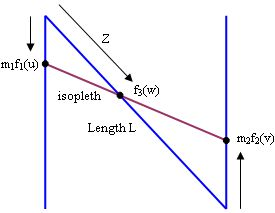
\includegraphics[width=0.2\textwidth]{./imagenes/geometry2.jpg}
    \end{figure} 

    se llama \textit{Gráfico N}, o más comúnmente, \textit{Gráfico Z} debido a 
    su forma. La escala media inclinada une a los valores de referencia de 
    las dos escalas externas (que se trazan en oposición). La línea media puede 
    inclinarse en cualquier dirección volteándo el diagrama y puede ser sólo una 
    sección parcial anclada en un extremo o flotando en el medio si no se 
    necesita toda la escala en el problema. El \textit{Gráfico Z} se puede usar
    para resolver una ecuación de $3$ variables de la forma 
    \begin{equation*}
        f_{3} (w) = \frac{f_{1} (u)}{f_{2} (v)}
    \end{equation*} 

    Por triángulos similares, tenemos que 
    \begin{equation*}
        \frac{m_{1}f_{1} (u)}{m_{2}f_{2} (v)} = \frac{Z}{[L-Z]}
    \end{equation*}
    
    Sustituyendo $f_{3} (w)$ por $\frac{f_{1} (u)}{f_{2} (v)}$ y reorganizando
    los términos obtenemos la distancia a lo largo de $Z$ para las marcas de 
    verificación correspondientes a $f_{3} (w)$:
    \begin{equation*}
        Z = \frac{L f_{3} (w)}{[\frac{m_{2}}{m_{1}} + f_{3} (w)]}
    \end{equation*}

    La escala $f_{3} (w)$ no tiene un factor de escala uniforme $m_{3}$ como 
    antes. El gráfico $Z$ realiza una división con escalas lineales para $u$ y
    $v$. Las escalas lineales del Gráfico $Z$ son mucho más adecuadas para 
    combinar una división con una suma/resta, que las escalas paralelas 
    compuestas con sus escalas logarítmicas. Además, tenemos un  gráfico $Z$ 
    para la multiplicación. También es posible deslizar las escalas externas 
    hacia arriba o hacia abajo sin cambiar la marca de espaciado de la 
    escala $Z$, ya que gira gracias a sus puntos finales (los triángulos 
    aún son similares), dando como resultado un \textit{nomograma} con una 
    escala $Z$ perpendicular. 

    \item \textbf{Gráficos proporcionales}
    
    Los gráficos proporcionales resuelven una ecuación de $4$ incógnitas del 
    tipo 
    \begin{equation*}
        \frac{f_{1} (u)}{f_{2} (v)} = \frac{f_{3} (w)}{f_{4} (t)}
    \end{equation*}

    Si tomamos el diagrama del gráfico $Z$ y un segundo isopleto que 
    intersecta la línea $Z$ en el mismo punto que el primero, entonces tenemos
    triángulos similares:
    \begin{equation*}
        \frac{m_1 f_{1} (u)}{m_2 f_{2} (v)} = 
        \frac{m_{3} f_{3} (w)}{m_{4} f_{4} (t)}
    \end{equation*}

    \begin{figure}[htb]
        \centering
        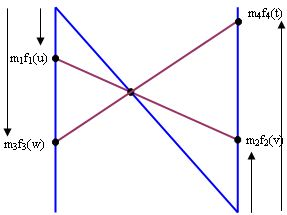
\includegraphics[width=0.2\textwidth]{./imagenes/geometry3.jpg}
    \end{figure} 

    que coincide con la ecuación anterior si elegimos la escala de las escalas 
    externas de modo que obtenemos
    \begin{equation*}
        \frac{m_1}{m_2} = \frac{m_{3}}{m_{4}}
    \end{equation*}

    Después, sobreponemos dos variables en cada escala exterior con esta 
    relación de factores de escalado, como se muestra en el siguiente 
    \textit{nomograma}:

    \begin{figure}[htb]
        \centering
        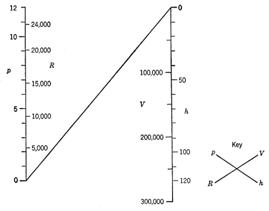
\includegraphics[width=0.2\textwidth]{./imagenes/image011.jpg}
        \caption{Nomograma de Josephs}
    \end{figure} 

    Otro tipo de gráfico proporcional utiliza líneas cruzadas dentro de un 
    área encuadrada. Por ejemplo, tomando los factores de escala anterior para 
    las cuatro variables están dados por 
    \begin{equation*}
        \frac{m_{1}}{m_{2}} = \frac{m_{3}}{m_4}
    \end{equation*} 

    donde éstos están relacionados como antes con las escalas $u, v, w$ y 
    $t$, respectivamente. 

    Pero hay otros tipos de gráficos proporcionales. En las etiquetas como 
    Tipo $3$, se dibuja una isopleta entre dos variables de escala, luego se 
    mueve en paralelo hasta que abarca el tercer valor de la variable y la 
    cuarta variable desconocida. En el \textit{nomograma de Tipo $4$}, la
    segunda isopleta se dibuja de manera perpendicular a la primera. 

    \begin{figure}[htb]
        \centering
        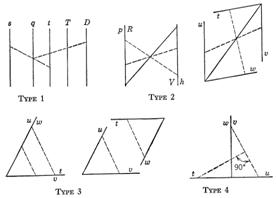
\includegraphics[width=0.2\textwidth]{./imagenes/image015.jpg}
    \end{figure} 

    \item \textbf{Gráficos de escala concurrente}
    
    El gráfico concurrente resuelve una ecuación del tipo 
    \begin{equation*}
        \frac{1}{f_{1} (u)} + \frac{1}{f_{2} (v)} = \frac{1}{f_{3} (w)}
    \end{equation*}

    La resistencia efectiva de dos resistencias paralelas está dada por esta 
    ecuación, y un \textit{nomograma de escala concurrente} de la forma 

    \begin{figure}[htb]
        \centering
        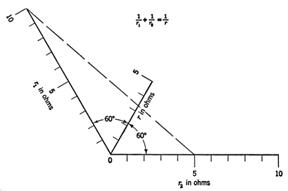
\includegraphics[width=0.3\textwidth]{./imagenes/image016.jpg}
    \end{figure} 
    
    La derivación es algo complicada, pero al final los factores de escala $m$
    deben cumplir las condiciones
    \begin{equation*}
        m_{1} = m_{2} = \frac{m_{3}}{2 \; cos (A)}
    \end{equation*}

    donde $A$ es el ángulo entre la escala $u$ y la escala $v$, y también el 
    ángulo entre la escala $v$ y la escala $w$. El factor de escala $m_{3}$
    corresponde a la escala $w$. Los ceros de las escalas deben encontrarse
    en el vértice. Por ejemplo, si se elige que el ángulo $A$ sea $60^{\circ}$
    entonces $2 \; cos (A) = 1$ y los tres factores de escala son idénticos,
    así como se muestra a continuación:
    \begin{figure}[htb]
        \centering
        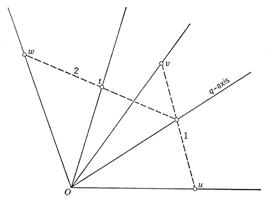
\includegraphics[width=0.3\textwidth]{./imagenes/image017.jpg}
    \end{figure} 

    Y para resolver la ecuación
    \begin{equation*}
        \frac{1}{f_{1} (u)} +  \frac{1}{f_{2} (v)} + \frac{1}{f_{4} (t)} =
        \frac{1}{f_{3} (w)}
    \end{equation*}

    se reorganiza como 
    \begin{equation*}
        \frac{1}{f_{1} (u)} + \frac{1}{f_{2} (v)} = 
        \frac{1}{f_{3} (w)} - \frac{1}{f_{4} (t)}
    \end{equation*}

    Después, las dos mitades se igualan a un valor intermedio $f_{q}$. Se crea 
    una escala concurrente compuesta de manera similar a otras escalas 
    compuestas como se muestra en la figura anterior (aquí se elige que 
    $A$ sea inferior a $60^{\circ}$). 

    \item \textbf{Gráficos de $4$ variables}

    Una ecuación de $4$ variables con una incógnita puede representarse como 
    una combinación de dos gráficos separados de cualquier tipo. Primero
    se divide la ecuación en dos partes en tres variables que son iguales 
    entre sí. Por ejemplo, para 
    \begin{equation*}
        f_{1} (u) + f_{2} (v) + f_{3} (w) = f_{4} (t)
    \end{equation*}

    y $t$ como incógnita, podemos reorganizar la ecuación en
    \begin{equation*}
        f_{1} (u) + f_{2} (v) = f_{4} (t) - f_{3} (w)
    \end{equation*}

    Se crea una variable $k$ para igualar esta suma. Luego se crea una
    \textit{escala en blanco} para $k$ para de tal forma que un 
    \textit{nomograma} de escala parelela para $f_{1} + f_{2} = k$ marca un 
    \textit{punto de pivote} en la escala de $k$. Se utiliza una segunda 
    alineación de regla desde este punto para $f_{4} - f_{3} = k$ para 
    encontrar $f_{4} (t)$. La escala para $u, v, w$ y la posición elegida para 
    la escala $k$ se pueden optimizar para minimizar los errores en el punto de
    pivote para pequeños errores en la alineación de la regla. 

    \begin{figure}[htb]
        \centering
        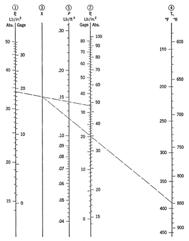
\includegraphics[width=0.2\textwidth]{./imagenes/image018.jpg}
    \end{figure} 
    
    \item \textbf{Gráficos de escala curva}
    
    Es posible derivar geométricamente relaciones para \textit{nomogramas} que 
    tienen una o más escalas curvas, pero el diseño de éstos es más sencillo si 
    se utilizan determinantes (esto es lo que abordan en la segunda parte del 
    ensayo). 
\end{enumerate}
\end{document} 